% !TEX program = xelatex
% 第三讲：从去噪到大模型
\documentclass[aspectratio=169,10pt,UTF8,fontset=none]{ctexbeamer}
% Preamble for this offering's decks.
% Lookup order for \input and figures: this folder, then ../shared/ (theme and
% slide-only figures), then ../../figures/ (the book's figures). `make slides`
% sets TEXINPUTS accordingly; \input@path covers compiling directly in this folder.
\makeatletter
\def\input@path{{../shared/}}
\makeatother
\usepackage{beamerthemegenai}
\graphicspath{{figures/}{../shared/figures/}{../../figures/}}

\title{生成模型与概率统计}
\author{张士欣}
\institute{中国科学院物理研究所}
\date{2026.10}
\renewcommand{\titlefigure}{cover_probability_flow.pdf}
\renewcommand*{\titleurl}{github.com/refraction-ray/free-energy-to-llms}

\subtitle{第三讲\quad 从去噪到大模型}
\renewcommand{\lecturename}{第三讲\quad 从去噪到大模型}

% A small "image" with additive noise: opacity of the picture, number of noise dots.
\newcommand{\noisytile}[3]{%
  \begin{scope}[shift={#1}]
    \begin{scope}
      \clip (0,0) rectangle (12,12);
      \fill[GMist] (0,0) rectangle (12,12);
      \begin{scope}[opacity=#2]
        \fill[GAmber] (0,0) rectangle (12,12);
        \fill[GOrange] (8.6,9) circle (1.7);
        \fill[GTeal] (-1,0) -- (4.3,6.8) -- (6.8,3.9) -- (9.4,6.4) -- (13,1.3) -- (13,0) -- cycle;
      \end{scope}
      \ifnum#3>0
        \foreach \j in {1,...,#3}{\fill[GSlate!80,opacity=0.75] (6+6*rand,6+6*rand) circle (0.33);}
      \fi
    \end{scope}
    \draw[GSlate!50] (0,0) rectangle (12,12);
  \end{scope}}

% Noised two-mode density: data 0.5 N(-2,0.3^2) + 0.5 N(2,0.3^2), x_t = a x_0 + b eps.
\pgfmathdeclarefunction{ptmix}{3}{%
  \pgfmathparse{0.5*(exp(-(#1+2*#2)^2/(2*(0.09*#2^2+#3^2)))+exp(-(#1-2*#2)^2/(2*(0.09*#2^2+#3^2))))/sqrt(2*pi*(0.09*#2^2+#3^2))}}
\pgfmathdeclarefunction{stmix}{3}{%
  \pgfmathparse{(-#1+2*#2*tanh(2*#2*#1/(0.09*#2^2+#3^2)))/(0.09*#2^2+#3^2)}}

\begin{document}

\begin{frame}[plain]
  \titlepage
\end{frame}

\begin{frame}{本讲路线}
  \begin{columns}[T]
    \begin{column}{0.5\textwidth}
      \textbf{上一讲留下的线索}
      \begin{itemize}
        \item 能量模型表达最自由，却被 MCMC 采样拖累
        \item score $\nabla_x\log p$ 与 $Z$ 无关，可以只用数据学
        \item 难点：数据附近之外 score 学不准，链也混合不动
      \end{itemize}
      \vspace{2mm}
      \textbf{本讲三部分}
      \begin{enumerate}
        \item 扩散模型：在许多噪声水平上学 score，把一次难采样拆成许多小步
        \item Transformer：大语言模型用来表示 $p(x_t\mid x_{<t})$ 的网络
        \item 大模型的训练阶段：从极大似然到带 KL 约束的奖励优化
      \end{enumerate}
    \end{column}
    \begin{column}{0.47\textwidth}
      \centering
      \begin{tikzpicture}[x=1mm,y=1mm]
        \pgfmathsetseed{4}
        \noisytile{(0,20)}{1}{0}
        \noisytile{(16,20)}{0.6}{35}
        \noisytile{(32,20)}{0.25}{80}
        \noisytile{(48,20)}{0}{140}
        \foreach \k in {0,1,2}{%
          \draw[arorange] (\k*16+12.3,34) to[bend left=30] (\k*16+15.7,34);
          \draw[arteal] (\k*16+15.7,18) to[bend left=30] (\k*16+12.3,18);}
        \node[lblo,anchor=south] at (30,37) {前向 $q$：逐步加噪（已知）};
        \node[lblt,anchor=north] at (30,15.5) {反向 $p_\theta$：逐步去噪（学习）};
        \node[lbl] at (6,8) {$x_0$};
        \node[lbl] at (54,8) {$x_T\approx\mathcal N(0,I)$};
      \end{tikzpicture}
    \end{column}
  \end{columns}
\end{frame}

% ====================================================================
\section{扩散、score 与 Flow Matching}

\begin{frame}{动机：一步太难，就拆成许多小步}
  \begin{columns}[T]
    \begin{column}{0.52\textwidth}
      \begin{itemize}
        \item GAN、VAE 想一步把噪声变成数据：映射极其复杂，或只能优化下界
        \item 能量模型用 Langevin 一步步走，但在多峰分布里混合极慢（上一讲：温度减半，慢 40 多倍）
        \item 扩散的思路：人为规定一个从数据走向噪声的过程，它每一步都很简单、完全已知；只学习它的反向
        \item 每一小步的反向转移近似是高斯，只需学一个“往哪里走”的方向
      \end{itemize}
      \vspace{1mm}
      \begin{concept}{贝叶斯公式}
        已知前向 $q(x_t\mid x_{t-1})$，反向 $q(x_{t-1}\mid x_t)\propto q(x_t\mid x_{t-1})\,q(x_{t-1})$；难算的部分只剩带噪数据的分布。
      \end{concept}
    \end{column}
    \begin{column}{0.45\textwidth}
      \begin{takeaway}[关键想法]
        高噪声时分布接近高斯，各个峰连成一片，像高温；低噪声时细节丰富，但相邻两步很接近。生成就像退火：从高温慢慢降下来，每一步只修正一点。
      \end{takeaway}
      \vspace{2mm}
      \small
      \begin{tabularx}{\linewidth}{@{}>{\color{GNavy}}l X@{}}
        \toprule
        2015 & 非平衡热力学视角的扩散概率模型\\
        2019 & 多噪声水平的 score 模型\\
        2020 & DDPM（去噪扩散概率模型）：噪声回归，图像质量追上 GAN\\
        2021 & 随机微分方程统一框架\\
        2022-- & 潜空间扩散、DiT（扩散 Transformer）、Flow Matching（流匹配）\\
        \bottomrule
      \end{tabularx}
    \end{column}
  \end{columns}
\end{frame}

\newcommand{\difpanel}[4]{%
  \begin{axis}[genai,#4,width=4.1cm,height=3.2cm,xmin=-4,xmax=4,ymin=0,ymax=0.75,xtick=\empty,ytick=\empty,domain=-4:4,samples=201,title={\scriptsize #3},title style={yshift=-1.2ex}]
    \addplot[GTeal,fill=GSky] {ptmix(x,#1,#2)} \closedcycle;
  \end{axis}}

\begin{frame}{前向加噪：任意时刻都有闭式解}
  \centering
  \begin{tikzpicture}
    \difpanel{1}{0.02}{$t=0$：数据}{name=a}
    \difpanel{0.92}{0.4}{$t$ 较小}{at={(a.east)},anchor=west,xshift=2mm,name=b}
    \difpanel{0.6}{0.8}{$t$ 较大}{at={(b.east)},anchor=west,xshift=2mm,name=c}
    \difpanel{0.1}{0.995}{$t=T$：近似 $\mathcal N(0,1)$}{at={(c.east)},anchor=west,xshift=2mm,name=d}
  \end{tikzpicture}
  \vspace{2mm}
  \begin{columns}[T]
    \begin{column}{0.52\textwidth}
      DDPM 每一步 $q(x_t\mid x_{t-1})=\mathcal N(\sqrt{1-\beta_t}\,x_{t-1},\beta_tI)$，合并后
      \[
        x_t=\underbrace{\sqrt{\bar\alpha_t}}_{a_t}\,x_0+\underbrace{\sqrt{1-\bar\alpha_t}}_{b_t}\,\epsilon,\quad \epsilon\sim\mathcal N(0,I)
      \]
      其中 $\bar\alpha_t=\prod_{s\le t}(1-\beta_s)$。训练时直接抽 $t,\epsilon$ 合成 $x_t$，无需逐步模拟。
    \end{column}
    \begin{column}{0.45\textwidth}
      \begin{concept}{高斯卷积}
        独立高斯之和仍是高斯，方差递推 $v_t=\alpha_tv_{t-1}+\beta_t$ 解得 $1-\bar\alpha_t$。带噪分布 $p_t$ 是数据分布与高斯核的卷积：峰被抹平、最终只剩一个高斯。
      \end{concept}
    \end{column}
  \end{columns}
\end{frame}

\begin{frame}{想一想：猜出加进去的噪声}
  \begin{columns}[c]
    \begin{column}{0.48\textwidth}
      \centering
      \begin{tikzpicture}[x=1.6mm,y=1.6mm]
        \pgfmathsetseed{4}
        \noisytile{(0,0)}{1}{0}
        \noisytile{(22,0)}{0.6}{35}
        \draw[arorange] (13,6) -- node[lblo,above] {$+\,b_t\epsilon$} (21,6);
        \node[lbl,anchor=north] at (6,-1) {原图 $x_0$};
        \node[lbl,anchor=north] at (28,-1) {带噪的 $x_t$};
        \node[font=\large\bfseries,text=GOrange] at (17,-6) {$\epsilon=\,?$};
      \end{tikzpicture}
      \par\vspace{3mm}
      {\small 训练时只把 $x_t$ 和 $t$ 交给网络，原图 $x_0$ 不给。}
    \end{column}
    \begin{column}{0.48\textwidth}
      \begin{hook}
        让网络从 $x_t$ 说出加进去的噪声 $\epsilon$。
        \par\medskip
        \opt{1}{这件事做得到吗？}
        \opt{2}{做不到的话，用均方误差训练，网络会学到什么？学到的东西有什么用？}
      \end{hook}
    \end{column}
  \end{columns}
\end{frame}

\begin{frame}{训练：让网络猜加进去的噪声}
  \begin{columns}[T]
    \begin{column}{0.5\textwidth}
      \begin{procedure}{训练：噪声回归}
        \begin{enumerate}\setlength{\itemsep}{0pt}
          \item 取数据 $x_0$，随机抽 $t$ 与 $\epsilon\sim\mathcal N(0,I)$
          \item 合成 $x_t=a_tx_0+b_t\epsilon$
          \item 最小化 $\|\epsilon-\epsilon_\theta(x_t,t)\|^2$
        \end{enumerate}
      \end{procedure}
      \vspace{1mm}
      {\small 网络输入 $x_t$ 与 $t$，所有 $t$ 共用一个网络（U-Net 或 Transformer）。猜出噪声即猜出原图：$\hat x_0=(x_t-b_t\epsilon_\theta)/a_t$。}
      \vspace{1mm}
      \begin{answer}
        第 1 问：做不到，同一个 $x_t$ 有多种可能的来历。均方回归的最优解是条件期望 $\E[\epsilon\mid x_t=x]$，网络学到的是后验平均（右图橙色）。它有什么用？见下一页。
      \end{answer}
    \end{column}
    \begin{column}{0.46\textwidth}
      \centering
      \begin{tikzpicture}[x=0.95mm,y=0.95mm]
        \fill[GSky] (0,0) circle (17);
        \node[circle,fill=GNavy,inner sep=0pt,minimum size=2mm,label={[lbln]below:$x_t$}] (x) at (0,0) {};
        \foreach \p/\w/\l in {(-14,9)/0.5/{$a_tx_0^{(1)}$},(12,11)/1.6/{$a_tx_0^{(2)}$},(13,-8)/0.9/{$a_tx_0^{(3)}$}}{%
          \node[dotT] (c) at \p {};
          \node[lblt,anchor=south,yshift=1mm] at \p {\l};
          \draw[-{Latex[length=1.4mm]},GTeal!60,line width=\w pt] (x) -- (c);}
        \draw[-{Latex[length=2mm]},GOrange,line width=1.6pt] (x) -- (6,5.5);
        \node[lblo,anchor=west] at (6.5,3.5) {$-b_t\,\E[\epsilon\mid x_t]$};
      \end{tikzpicture}
      \par\vspace{1mm}
      {\scriptsize\slate{同一个 $x_t$ 可能来自不同原图。青色：若原图是 $x_0^{(k)}$，去噪方向是 $-b_t\epsilon^{(k)}$，粗细表示后验 $p(x_0^{(k)}\mid x_t)$；橙色：网络学到的后验平均}}
    \end{column}
  \end{columns}
\end{frame}

\begin{frame}{为什么预测噪声就是在学 score}
  \begin{columns}[T]
    \begin{column}{0.56\textwidth}
      \begin{keystep}
        带噪分布是高斯混合，$q(x\mid x_0)=\mathcal N(a_tx_0,b_t^2I)$：
        \keyeq{p_t(x)=\int p_{\mathrm{data}}(x_0)\,q(x\mid x_0)\,dx_0}
        对 $x$ 求梯度，并利用 $\nabla q=q\,\nabla\log q$：
        \keyeq{\nabla\log p_t(x)&=\int\underbrace{\frac{p_{\mathrm{data}}(x_0)\,q(x\mid x_0)}{p_t(x)}}_{\text{后验 }p(x_0\mid x_t=x)}\,\nabla\log q\,dx_0\\
          &=\E\Bigl[-\frac{x-a_tx_0}{b_t^2}\Bigm| x_t=x\Bigr]\\
          &=-\frac{1}{b_t}\,\E[\epsilon\mid x_t=x]}
        即各张原图的 score 按后验加权平均（用了 $x-a_tx_0=b_t\epsilon$）。对照上一页：
        \keyeq{s_t(x)\approx-\epsilon_\theta(x,t)/b_t}
      \end{keystep}
    \end{column}
    \begin{column}{0.41\textwidth}
      \centering
      \begin{tikzpicture}
        \begin{axis}[genai,name=d,width=5.9cm,height=2.6cm,xmin=-3.5,xmax=3.5,ymin=0,ymax=0.36,xtick=\empty,ytick=\empty,domain=-3.5:3.5,samples=161]
          \addplot[GTeal,fill=GSky] {0.5*(exp(-(x+1.6)^2/0.72)+exp(-(x-1.6)^2/0.72))/sqrt(0.72*pi)} \closedcycle;
          \node[lblt,anchor=west] at (axis cs:2.3,0.25) {$p_t$};
        \end{axis}
        \begin{axis}[genai,at={(d.south)},anchor=north,yshift=-1mm,width=5.9cm,height=3.3cm,xmin=-3.5,xmax=3.5,ymin=-10,ymax=10,xtick={-1.6,1.6},xticklabels={$-2a_t$,$2a_t$},ytick={0},domain=-3.5:3.5,samples=301,restrict y to domain=-12:12]
          \addplot[GSlate!50,line width=0.5pt] {0};
          \addplot[GSlate,dashed,line width=0.7pt] {-(x+1.6)/0.36};
          \addplot[GSlate,dashed,line width=0.7pt] {-(x-1.6)/0.36};
          \addplot[GOrange] {(-x+1.6*tanh(4.444*x))/0.36};
          \node[lbl,anchor=north east] at (axis cs:0.7,-7.2) {$x_0=-2$};
          \node[lbl,anchor=south west] at (axis cs:-0.7,7.2) {$x_0=2$};
          \node[lblo,anchor=west] at (axis cs:0.3,4.6) {$s_t$};
        \end{axis}
      \end{tikzpicture}
      \par\vspace{1mm}
      {\scriptsize\slate{数据只有 $x_0=\pm2$ 两点（$a_t=0.8$，$b_t=0.6$）。虚线：两张原图各自的条件 score；橙色：总 score，按后验权重在两者之间切换}}
      \vspace{2mm}
      \begin{answer}
        这个后验平均恰好就是 score。不用算 $Z$，也没有散度项，只做去噪回归。
      \end{answer}
    \end{column}
  \end{columns}
\end{frame}

\begin{frame}{采样：从噪声一步步走回数据}
  \begin{columns}[T]
    \begin{column}{0.5\textwidth}
      {\small 前向是一条已知的马尔可夫链 $x_0\to x_1\to\cdots\to x_T$。采样就是倒着走：每一步从反向转移 $q(x_{t-1}\mid x_t)$ 抽一个样本。}
      \vspace{1mm}
      \begin{procedure}{采样：逐步去噪}
        \begin{enumerate}\setlength{\itemsep}{0pt}
          \item $x_T\sim\mathcal N(0,I)$
          \item 对 $t=T,\ldots,1$：抽 $z\sim\mathcal N(0,I)$（$t=1$ 时取 $z=0$），
            \[x_{t-1}=\underbrace{\frac{1}{\sqrt{\alpha_t}}\Bigl(x_t-\frac{\beta_t}{b_t}\epsilon_\theta(x_t,t)\Bigr)}_{\text{均值 }\mu_\theta(x_t)}+\sigma_tz\]
          \item 输出 $x_0$。共调用网络 $T$ 次（DDPM 中 $T=1000$）
        \end{enumerate}
      \end{procedure}
    \end{column}
    \begin{column}{0.46\textwidth}
      \centering
      \begin{tikzpicture}[x=1mm,y=1mm]
        \pgfmathsetseed{4}
        \noisytile{(0,20)}{0}{140}
        \noisytile{(17,20)}{0.25}{80}
        \noisytile{(34,20)}{0.6}{35}
        \noisytile{(51,20)}{1}{0}
        \foreach \k in {0,1,2}{\draw[arteal] (\k*17+12.3,26) -- (\k*17+16.7,26);}
        \node[lbl] at (6,17) {$x_T$};
        \node[lbl] at (23,17) {$x_t$};
        \node[lbl] at (40,17) {$x_{t-1}$};
        \node[lbl] at (57,17) {$x_0$};
        \node[lblt,anchor=south] at (31.5,33) {每个箭头：从 $q(x_{t-1}\mid x_t)$ 抽一次};
        \draw[GSlate!50,densely dashed] (23,14.5) -- (2,9.5);
        \draw[GSlate!50,densely dashed] (40,14.5) -- (61,9.5);
        \node[nteal,font=\scriptsize,minimum height=6mm,inner sep=1.5pt] (a) at (5,4) {$x_t$};
        \node[norange,font=\scriptsize,minimum height=6mm,inner sep=1.5pt] (b) at (22,4) {网络 $\epsilon_\theta$};
        \node[nsoft,font=\scriptsize,minimum height=6mm,inner sep=1.5pt] (c) at (40,4) {均值 $\mu_\theta$};
        \node[nteal,font=\scriptsize,minimum height=6mm,inner sep=1.5pt] (d) at (58,4) {$x_{t-1}$};
        \draw[ar] (a) -- (b);
        \draw[ar] (b) -- (c);
        \draw[ar] (c) -- node[lbl,above] {$+\sigma_tz$} (d);
      \end{tikzpicture}
      \par\vspace{1mm}
      {\scriptsize\slate{上：生成方向，噪声逐步变成图像。下：放大其中一步}}
      \vspace{2mm}
      \begin{concept}{高斯近似}
        步长 $\beta_t$ 很小时，反向一步近似高斯，只需知道均值和方差。方差 $\sigma_t^2$ 由噪声调度定好；均值由网络算出，公式从哪来见下一页。
      \end{concept}
    \end{column}
  \end{columns}
\end{frame}

\begin{frame}{反向一步：先猜原图，再朝它挪一小步}
  \begin{columns}[T]
    \begin{column}{0.55\textwidth}
      \begin{keystep}
        \textbf{假如知道原图 $x_0$}：由贝叶斯公式
        \keyeq{q(x_{t-1}\mid x_t,x_0)\propto\underbrace{q(x_t\mid x_{t-1})}_{\text{前向一步}}\;\underbrace{q(x_{t-1}\mid x_0)}_{\text{闭式加噪}}}
        两个因子都是 $x_{t-1}$ 的高斯，乘积仍是高斯，均值是 $x_t$ 与 $x_0$ 的加权组合：
        \keyeq{\tilde\mu_t=\underbrace{\frac{\sqrt{\alpha_t}\,b_{t-1}^2}{b_t^2}}_{\approx1}\,x_t+\underbrace{\frac{a_{t-1}\beta_t}{b_t^2}}_{\text{很小}}\,x_0,\qquad\tilde\beta_t=\frac{b_{t-1}^2}{b_t^2}\,\beta_t}
        \textbf{不知道 $x_0$}：代入网络的估计 $\hat x_0=(x_t-b_t\epsilon_\theta)/a_t$，化简得：
        \keyeq{\mu_\theta(x_t)=\frac{1}{\sqrt{\alpha_t}}\Bigl(x_t-\frac{\beta_t}{b_t}\,\epsilon_\theta(x_t,t)\Bigr),\qquad\sigma_t^2=\tilde\beta_t}
      \end{keystep}
      {\small 这正是上一页算法里的均值。$\tilde\mu_t$ 对 $x_0$ 线性，由全期望公式，代入 $\E[x_0\mid x_t]$ 恰好得到 $\E[x_{t-1}\mid x_t]$。}
    \end{column}
    \begin{column}{0.42\textwidth}
      \centering
      \begin{tikzpicture}[x=1mm,y=1mm]
        \pgfmathsetseed{4}
        \noisytile{(0,30)}{0.3}{90}
        \noisytile{(44,30)}{0.8}{0}
        \noisytile{(22,0)}{0.38}{75}
        \node[lbl,anchor=north] at (6,29) {$x_t$};
        \node[lblt,anchor=south] at (50,43) {猜出的原图 $\hat x_0$};
        \node[lbl,anchor=north] at (28,-1) {$x_{t-1}$};
        \draw[arteal] (13,36) -- node[lblt,above] {网络 $\epsilon_\theta$} (43,36);
        \draw[ar,line width=1.6pt] (8,29.5) -- node[lbl,left,pos=0.45] {大部分} (23,12.5);
        \draw[arorange,line width=0.5pt] (48,29.5) -- node[lblo,right,pos=0.45] {一小步} (33,12.5);
        \node[lblo,anchor=west] at (34.5,4) {$+\,\sigma_tz$};
      \end{tikzpicture}
      \par\vspace{2mm}
      {\scriptsize\slate{每一步：网络先从 $x_t$ 猜出原图 $\hat x_0$（只是后验平均，比较模糊），再把 $x_t$ 朝 $\hat x_0$ 挪一小步，加一点噪声。猜得粗没关系，下一步会在更清楚的图上重新猜}}
    \end{column}
  \end{columns}
\end{frame}

\begin{frame}{串起来：一个网络，三种读法}
  \centering
  \begin{tikzpicture}[x=1mm,y=0.93mm,
      box/.style={font=\scriptsize,minimum height=9mm,align=flush center,inner sep=1.6pt},
      el/.style={lbl,fill=white,inner sep=0.8pt}]
    \node[lbln,font=\footnotesize\bfseries] at (15,47.5) {训练};
    \node[nsoft,box,text width=28mm] (fw) at (15,38) {前向加噪（已知、闭式）\\$x_t=a_tx_0+b_t\epsilon$};
    \node[norange,box,text width=28mm] (tr) at (15,8) {噪声回归\\$\min\E\|\epsilon-\epsilon_\theta(x_t,t)\|^2$};
    \draw[ar] (fw) -- node[el,align=center] {合成训练对\\$(x_t,\epsilon)$} (tr);
    \node[lbln,font=\footnotesize\bfseries] at (64,47.5) {网络学到的：给定 $x_t$ 的后验平均};
    \node[nteal,box,text width=42mm] (eps) at (64,38) {噪声\\$\epsilon_\theta\approx\E[\epsilon\mid x_t]$};
    \node[nteal,box,text width=42mm] (x0) at (64,23) {原图\\$\hat x_0=(x_t-b_t\epsilon_\theta)/a_t\approx\E[x_0\mid x_t]$};
    \node[nteal,box,text width=42mm] (sc) at (64,8) {score\\$s_t=-\epsilon_\theta/b_t\approx\nabla\log p_t$};
    \draw[ar] (tr.east) -- node[el,pos=0.45] {条件期望} (eps.west);
    \draw[GTeal,line width=0.7pt,{Latex[length=1.4mm]}-{Latex[length=1.4mm]}] (eps) -- node[el] {线性换算} (x0);
    \draw[GTeal,line width=0.7pt,{Latex[length=1.4mm]}-{Latex[length=1.4mm]}] (x0) -- node[el] {高斯混合求导} (sc);
    \node[lbln,font=\footnotesize\bfseries] at (116,47.5) {采样};
    \node[nnavy,box,text width=40mm] (step) at (116,38) {反向一步\\\mbox{$x_{t-1}=\frac{1}{\sqrt{\alpha_t}}\bigl(x_t-\frac{\beta_t}{b_t}\epsilon_\theta\bigr)+\sigma_tz$}};
    \node[nnavy,box,text width=40mm] (bay) at (116,23) {贝叶斯：已知 $x_0$ 时\\$q(x_{t-1}\mid x_t,x_0)$ 是高斯，代入 $\hat x_0$};
    \node[nnavy,box,text width=40mm] (lan) at (116,8) {代入 $s_t$ 改写：\mbox{$x_{t-1}=\frac{x_t+\beta_ts_t}{\sqrt{\alpha_t}}+\sigma_tz$}\\连续极限：反向 SDE、概率流 ODE};
    \draw[ar] (x0.east) -- (bay.west);
    \draw[ar] (sc.east) -- (lan.west);
    \draw[ar] (bay) -- (step);
    \draw[GSlate,line width=0.75pt,{Latex[length=1.7mm,width=1.35mm]}-{Latex[length=1.7mm,width=1.35mm]}] (lan.east) -- ++(3,0) |- (step.east);
  \end{tikzpicture}
  \par
  {\scriptsize\slate{用到的概率工具：高斯卷积（前向）\quad 条件期望（训练）\quad 混合分布的梯度（score）\quad 贝叶斯公式与全期望公式（采样）}}
  \vfill
  \begin{takeaway}
    噪声、原图、score 只差线性换算，都是给定 $x_t$ 的后验平均。训练只用条件期望；采样一步由贝叶斯公式推出，换成 score 写，连续极限就是后面的 SDE 与 ODE。
  \end{takeaway}
\end{frame}

\begin{frame}{不同噪声水平的 score}
  \centering
  \begin{tikzpicture}
    \begin{axis}[genai,name=a,width=4.6cm,height=2.9cm,xmin=-4,xmax=4,ymin=0,ymax=0.75,xtick=\empty,ytick=\empty,domain=-4:4,samples=201,title={\scriptsize 低噪声},title style={yshift=-1.2ex}]
      \addplot[GTeal,fill=GSky] {ptmix(x,0.97,0.25)} \closedcycle;
    \end{axis}
    \begin{axis}[genai,name=b,at={(a.east)},anchor=west,xshift=4mm,width=4.6cm,height=2.9cm,xmin=-4,xmax=4,ymin=0,ymax=0.75,xtick=\empty,ytick=\empty,domain=-4:4,samples=201,title={\scriptsize 中等噪声},title style={yshift=-1.2ex}]
      \addplot[GTeal,fill=GSky] {ptmix(x,0.8,0.6)} \closedcycle;
    \end{axis}
    \begin{axis}[genai,name=c,at={(b.east)},anchor=west,xshift=4mm,width=4.6cm,height=2.9cm,xmin=-4,xmax=4,ymin=0,ymax=0.75,xtick=\empty,ytick=\empty,domain=-4:4,samples=201,title={\scriptsize 高噪声},title style={yshift=-1.2ex}]
      \addplot[GTeal,fill=GSky] {ptmix(x,0.4,0.92)} \closedcycle;
    \end{axis}
    \foreach \n/\a/\b in {a/0.97/0.25,b/0.8/0.6,c/0.4/0.92}{%
      \begin{axis}[genai,at={(\n.south)},anchor=north,yshift=-1mm,width=4.6cm,height=2.9cm,xmin=-4,xmax=4,ymin=-7,ymax=7,xtick=\empty,ytick={0},domain=-4:4,samples=301]
        \addplot[GSlate!50,line width=0.5pt] {0};
        \addplot[GOrange] {stmix(x,\a,\b)};
      \end{axis}}
    \node[lblt,anchor=east] at ([xshift=-2mm,yshift=-4mm]a.west) {$p_t$};
    \node[lblo,anchor=east] at ([xshift=-2mm,yshift=-26mm]a.west) {$s_t$};
  \end{tikzpicture}
  \vspace{2mm}
  \begin{takeaway}
    低噪声时 score 精细而陡峭，只在数据附近可靠；高噪声时 score 平滑，几乎是指向原点的线性场。采样从高噪声出发，先定大致位置，再逐级补细节，这避开了单一 score 在数据远处学不准、混合慢的问题。
  \end{takeaway}
\end{frame}

\begin{frame}{连续时间：随机微分方程与概率流}
  \begin{columns}[T]
    \begin{column}{0.48\textwidth}
      正向加噪写成随机微分方程（SDE）：$dx=f(x,t)\,dt+g(t)\,dW_t$。
      \begin{itemize}
        \item 反向 SDE（随机）：
          $dx=\bigl[f-g^2\,s_t(x)\bigr]dt+g\,d\bar W_t$
        \item 概率流 ODE（确定）：
          $\dfrac{dx}{dt}=f-\tfrac12g^2\,s_t(x)$
      \end{itemize}
      两者在每个时刻的边缘分布 $p_t$ 都相同，单条轨迹不同。缺的只有 score，正好由噪声网络给出。
      \vspace{1mm}
      \begin{concept}{Fokker--Planck 方程}
        密度演化中的扩散项可以改写成输运：$\partial_tp=-\nabla\cdot\bigl[(f-\tfrac12g^2s)\,p\bigr]$，这就是概率流 ODE 的来历。
      \end{concept}
    \end{column}
    \begin{column}{0.5\textwidth}
      \centering
      \begin{tikzpicture}[x=26mm,y=5.2mm]
        \begin{scope}
          \clip (0,-3.5) rectangle (1,3.5);
          \input{figures/diff_sde.tex}
        \end{scope}
        \draw[GSlate!60] (0,-3.5) rectangle (1,3.5);
        \node[lblo,anchor=south] at (0.5,3.6) {反向 SDE};
        \begin{scope}[shift={(1.12,0)}]
          \begin{scope}
            \clip (0,-3.5) rectangle (1,3.5);
            \input{figures/diff_ode.tex}
          \end{scope}
          \draw[GSlate!60] (0,-3.5) rectangle (1,3.5);
          \node[lblt,anchor=south] at (0.5,3.6) {概率流 ODE};
        \end{scope}
        \node[lbl,anchor=north] at (0.5,-3.6) {噪声 $\rightarrow$ 数据};
        \node[lbl,anchor=north] at (1.62,-3.6) {噪声 $\rightarrow$ 数据};
      \end{tikzpicture}
      \par\vspace{1mm}
      {\scriptsize\slate{横轴为生成时间。两种轨迹都落到两个模式上，ODE 轨迹互不相交}}
    \end{column}
  \end{columns}
\end{frame}

\begin{frame}{想一想：直线训练，学出什么轨迹}
  \begin{columns}[c]
    \begin{column}{0.4\textwidth}
      \centering
      \begin{tikzpicture}[x=34mm,y=7mm]
        \begin{scope}
          \clip (0,-3.2) rectangle (1,3.2);
          \input{figures/fm_lines.tex}
        \end{scope}
        \draw[GSlate!60] (0,-3.2) rectangle (1,3.2);
        \node[lbl,anchor=north] at (0.5,-3.3) {$r:0\rightarrow1$};
        \node[lbl,anchor=south] at (0,3.3) {噪声 $z$};
        \node[lbl,anchor=south] at (1,3.3) {数据 $y$};
      \end{tikzpicture}
    \end{column}
    \begin{column}{0.56\textwidth}
      另一种训练方式 Flow Matching（流匹配）：随机配对噪声 $z$ 与数据 $y$，连成直线 $x_r=(1-r)z+ry$；在直线上任取一点，让网络回归这条直线的速度 $y-z$。
      \vspace{3mm}
      \begin{hook}
        训练用的全是直线，而且互相交叉。用学到的速度场生成时，轨迹是什么样？
        \par\medskip
        \opt{A}{直线，会交叉}
        \opt{B}{直线，互不相交}
        \opt{C}{弯曲，互不相交}
      \end{hook}
    \end{column}
  \end{columns}
\end{frame}

\begin{frame}{Flow Matching：直接学速度}
  \begin{columns}[T]
    \begin{column}{0.5\textwidth}
      取噪声 $z$ 与数据 $y$，走直线 $x_r=(1-r)z+ry$，它的速度是 $y-z$：
      \setlength{\abovedisplayskip}{4pt}\setlength{\belowdisplayskip}{4pt}%
      \[
        \mathcal L=\E_{y,z,r}\bigl\|v_\theta(x_r,r)-(y-z)\bigr\|^2
      \]
      \begin{itemize}
        \item 同一个 $x_r$ 可能来自许多对 $(z,y)$；最优解是条件平均 $v_r(x)=\E[y-z\mid x_r=x]$
        \item 训练只需随机取一个时刻做回归，不解任何 ODE
        \item 生成：$z\sim\mathcal N(0,I)$，沿 $dx/dr=v_\theta$ 积分到 $r=1$
      \end{itemize}
      \begin{concept}{条件期望}
        和噪声回归同一个原理：对单对样本的回归，学到总体的速度场。
      \end{concept}
    \end{column}
    \begin{column}{0.47\textwidth}
      \centering
      \begin{tikzpicture}[x=26mm,y=6mm]
        \begin{scope}
          \clip (0,-3.2) rectangle (1,3.2);
          \input{figures/fm_lines.tex}
        \end{scope}
        \draw[GSlate!60] (0,-3.2) rectangle (1,3.2);
        \node[lbl,anchor=south] at (0.5,3.3) {训练：随机配对的直线};
        \begin{scope}[shift={(1.12,0)}]
          \begin{scope}
            \clip (0,-3.2) rectangle (1,3.2);
            \input{figures/fm_traj.tex}
          \end{scope}
          \draw[GSlate!60] (0,-3.2) rectangle (1,3.2);
          \node[lblt,anchor=south] at (0.5,3.3) {生成：学到的流线};
        \end{scope}
        \node[lbl,anchor=north] at (0.5,-3.3) {$r:0\rightarrow1$};
        \node[lbl,anchor=north] at (1.62,-3.3) {$r:0\rightarrow1$};
      \end{tikzpicture}
      \par\vspace{2mm}
      \begin{answer}
        C。ODE 的解唯一，流线不能相交。在训练直线交叉的地方，网络只能输出各条直线速度的平均，流线因此弯开。
      \end{answer}
    \end{column}
  \end{columns}
\end{frame}

\begin{frame}{Flow Matching 与连续归一化流（CNF）：同一个模型，两种训练}
  \centering
  \resizebox{\textwidth}{!}{\begin{tikzpicture}[x=1mm,y=1mm]
    \node[lbln,anchor=west,font=\footnotesize\bfseries] at (0,32) {CNF：极大似然训练};
    \node[nteal,minimum width=24mm] (n1) at (13,24) {数据 $x$};
    \node[norange,minimum width=38mm,font=\scriptsize] (n2) at (52,24) {ODE 求解器：$r=1\to0$ 反向积分\\同时累积散度 $\int\nabla\cdot v_\theta\,dr$\\每个样本数十至上百次网络调用};
    \node[nsoft,minimum width=34mm,font=\scriptsize] (n3) at (96,24) {$-\log p_1(x)=-\log p_0(z)$\\$\qquad+\int_0^1\nabla\cdot v_\theta\,dr$};
    \node[nrose,minimum width=20mm,font=\scriptsize] (n4) at (132,24) {反向传播穿过\\整个求解过程};
    \draw[ar] (n1) -- (n2); \draw[ar] (n2) -- (n3); \draw[ar] (n3) -- (n4);
    \node[lbln,anchor=west,font=\footnotesize\bfseries] at (0,13) {Flow Matching：回归训练};
    \node[nteal,minimum width=22mm,font=\scriptsize] (m1) at (13,5) {$y\sim$ 数据\\$z\sim\mathcal N(0,I)$，$r\sim U[0,1]$};
    \node[nteal,minimum width=38mm,font=\scriptsize] (m2) at (52,5) {解析构造\\$x_r=(1-r)z+ry$，标签 $y-z$};
    \node[norange,minimum width=34mm,font=\scriptsize] (m3) at (96,5) {一次网络调用\\$v_\theta(x_r,r)$};
    \node[norange,minimum width=20mm,font=\scriptsize] (m4) at (132,5) {$\|v_\theta-(y-z)\|^2$\\普通回归};
    \draw[ar] (m1) -- (m2); \draw[ar] (m2) -- (m3); \draw[ar] (m3) -- (m4);
    \node[nnavy,minimum width=144mm,font=\scriptsize] at (71,-8) {推理（两者完全相同）：$z\sim\mathcal N(0,I)$，数值积分 $dx/dr=v_\theta(x,r)$ 得到样本；需要密度时同样沿轨迹积分散度};
  \end{tikzpicture}}
  \vfill
  \begin{takeaway}
    训练从“每个样本解一次 ODE、积分散度、对整条轨迹反传”变成“随机取一个时刻、做一次回归”；学到的速度场和生成 ODE 与 CNF 完全相同。要学一个把高斯搬运成数据的速度场，训练时却不必模拟这个搬运；连续时间流因此能扩展到图像、视频等高维数据。
  \end{takeaway}
\end{frame}

\newcommand{\riverpanel}[4]{%
  \begin{scope}[shift={(#1,0)}]
    \node[anchor=south west,inner sep=0pt] at (0,-3.5) {\includegraphics[width=30mm,height=30.8mm]{#2}};
    \begin{scope}
      \clip (0,-3.5) rectangle (1,3.5);
      #3
    \end{scope}
    \draw[GSlate!60] (0,-3.5) rectangle (1,3.5);
    \node[lbln,anchor=south,font=\scriptsize\bfseries] at (0.5,3.6) {#4};
  \end{scope}}

\begin{frame}{全景：一条概率之河}
  \begingroup\small 这几种方法做的是同一件事：选一条从高斯连续变到数据的概率路径 $p_t$，学一个向量场，让样本顺着它走回数据。下图横轴是生成时间（左为噪声，右为数据），纵轴是 $x$，颜色是 $p_t(x)$。\par\endgroup
  \par\vspace{1mm}
  \centering
  \begin{tikzpicture}[x=30mm,y=4.4mm]
    \riverpanel{0}{river_diff.png}{\input{figures/river_fwd.tex}}{1\enspace 加噪：河由数据吹散而成}
    \riverpanel{1.12}{river_diff.png}{\input{figures/river_score.tex}}{2\enspace score：河面的坡度}
    \riverpanel{2.24}{river_diff.png}{\input{figures/diff_sde.tex}\input{figures/diff_ode.tex}}{3\enspace 扩散采样：逆流走回}
    \riverpanel{3.36}{river_fm.png}{\input{figures/fm_traj.tex}\begin{scope}[opacity=0.8]\input{figures/fm_lines.tex}\end{scope}}{4\enspace Flow Matching：换一条直河}
    \foreach \k/\t in {0/{从数据向噪声扩散，已知},1.12/{箭头 $\nabla\log p_t$ 指向密度高处},2.24/{\orange{橙}：反向 SDE；\teal{青}：概率流 ODE},3.36/{灰：训练直线；\teal{青}：学到的流线}}{%
      \node[lbl,anchor=north,text width=31mm] at (\k+0.5,-3.65) {\t};}
  \end{tikzpicture}
  \par\vspace{1mm}
  \footnotesize
  \begin{tabularx}{\linewidth}{@{}>{\color{GNavy}\bfseries}l X X X@{}}
    \toprule
    & 河（概率路径） & 网络学什么 & 怎么走回数据\\
    \midrule
    扩散 & 逐步加噪 $x_t=a_tx_0+b_t\epsilon$ & score，即河面的坡度 & 反向 SDE 或概率流 ODE\\
    Flow Matching & 直线插值 $x_r=(1-r)z+ry$ & 速度，即水流本身 & 沿速度场积分 ODE\\
    \bottomrule
  \end{tabularx}
\end{frame}


\begin{frame}{扩散：小结}
  \centering
  \fourcard%
    {各噪声水平的 score $\nabla_x\log p_t$\\（或噪声、速度）}%
    {噪声 / score / 速度的均方回归\\负 ELBO 的重加权}%
    {从高斯出发，反向 SDE 或 ODE\\数十到上千次网络调用}%
    {采样步数多；似然需另行积分}
  \vfill
  \begin{takeaway}
    扩散绕开了 $Z$（只学梯度），绕开了混合慢（噪声把各模式连通），也避开了对抗博弈（训练只是回归）。代价是采样要多步。文本也可以做“掩码扩散”：前向把 token 逐步换成 [MASK]，反向逐步填回，这与下面 BERT 的完形填空相连。
  \end{takeaway}
\end{frame}

% ====================================================================
\section{Transformer：怎样表示 $p(x_t\mid x_{<t})$}

\begin{frame}{动机：需要一个读前缀、出分布的网络}
  \begin{columns}[T]
    \begin{column}{0.5\textwidth}
      自回归模型要一个函数：输入任意长的前缀 $x_{<t}$，输出词表上的分布。
      \begin{itemize}
        \item \textbf{n-gram}：只看前 $n-1$ 个 token，查频率表；上下文短，表随 $n$ 指数增长
        \item \textbf{循环网络}：把历史压进一个向量，逐个更新；训练也只能串行，长距离信息易丢失
        \item \textbf{Transformer}（2017）：每个位置直接按内容读取所有可见位置；训练时所有位置并行
      \end{itemize}
      \begin{concept}{马尔可夫假设}
        n-gram 是 $n-1$ 阶马尔可夫链；Transformer 不做截断，条件是整个前缀。
      \end{concept}
    \end{column}
    \begin{column}{0.47\textwidth}
      \centering
      \begin{tikzpicture}[x=1mm,y=1mm]
        \foreach \i/\w in {0/猫,1/坐,2/在,3/垫子,4/上}{\node[nsoft,minimum width=9mm] (t\i) at (\i*11,0) {\w};}
        \node[norange,minimum width=12mm] (q) at (55,0) {?};
        \foreach \i/\w in {0/0.6,1/0.6,2/0.9,3/1.5,4/1.1}{\draw[arteal,line width=\w pt] (t\i.north) to[bend left=35] (q.north);}
        \node[lblt,anchor=south] at (31,13) {每个位置直接读取全部前缀};
        \foreach \i in {0,...,3}{\draw[ar] (\i*11,-8) -- (\i*11+11,-8);}
        \draw[ar] (44,-8) -- (55,-8);
        \node[lbl,anchor=north] at (27.5,-10) {循环网络：信息逐个传递};
      \end{tikzpicture}
    \end{column}
  \end{columns}
\end{frame}

\begin{frame}{从文字到向量}
  \centering
  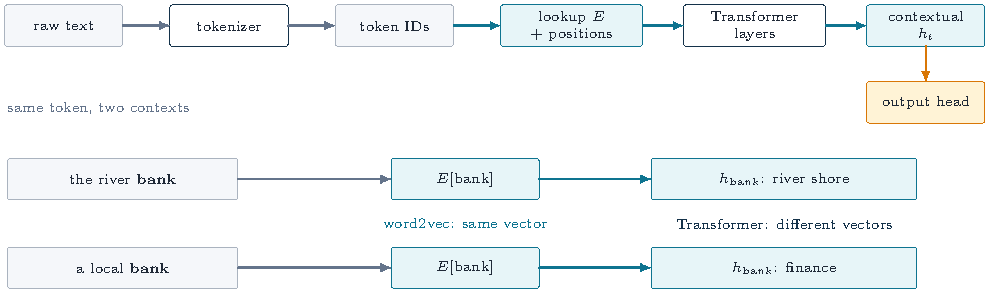
\includegraphics[width=0.95\textwidth]{token_to_context.pdf}
  \vfill
  \begin{itemize}
    \item 分词器把文字切成 token 编号；编号只是类别标签，大小没有含义
    \item 嵌入矩阵 $E\in\R^{|\mathcal V|\times d}$ 为每个编号查一行向量；它与模型一起由训练损失更新
    \item 查表向量与上下文无关；经过 Transformer 层后，同一个 token 在不同句子中得到不同的表示
  \end{itemize}
\end{frame}

\begin{frame}{注意力：按内容加权平均}
  \begin{columns}[c]
    \begin{column}{0.56\textwidth}
      \centering
      \begin{tikzpicture}[x=1mm,y=1mm]
        \foreach \i/\w/\a in {0/猫/0.10,1/坐/0.05,2/在/0.10,3/垫子/0.60,4/上/0.15}{%
          \node[nsoft,minimum width=9mm,font=\scriptsize] (t\i) at (\i*12,0) {\w};
          \node[nteal,minimum width=8mm,minimum height=5mm,font=\scriptsize] (k\i) at (\i*12,10) {$k_{\i}$};
          \fill[GOrange!80] (\i*12-3,16) rectangle ++(6,\a*28);
          \node[font=\tiny,text=GSlate] at (\i*12,\a*28+18) {\a};
          \node[nteal,minimum width=8mm,minimum height=5mm,font=\scriptsize] (v\i) at (\i*12,-10) {$v_{\i}$};
          \draw[GSlate!50] (t\i) -- (k\i);
          \draw[GSlate!50] (t\i) -- (v\i);}
        \node[norange,minimum width=10mm,font=\scriptsize] (q) at (-16,19) {$q_t$};
        \draw[arorange] (q.east) -- ++(7,0);
        \node[lblo,anchor=north] at (-16,14) {当前位置的查询};
        \node[lblo,anchor=south west] at (-9,36) {$a_{tj}=\softmax_j\bigl(q_t\cdot k_j/\sqrt{d_k}\bigr)$};
        \node[norange,font=\scriptsize] (o) at (24,-24) {$o_t=\sum_ja_{tj}v_j$};
        \foreach \i/\w in {0/0.4,1/0.3,2/0.4,3/1.4,4/0.6}{\draw[GOrange,line width=\w pt] (v\i.south) -- (o.north);}
      \end{tikzpicture}
    \end{column}
    \begin{column}{0.41\textwidth}
      \begin{itemize}
        \item query $q$：当前位置“想找什么”
        \item key $k$：每个位置“按什么被检索”
        \item value $v$：被读取的内容
        \item 三者都是同一表示经不同矩阵投影：$Q=XW_Q$，$K=XW_K$，$V=XW_V$
      \end{itemize}
      \begin{concept}{期望}
        权重 $a_{t\cdot}$ 是位置上的一个 categorical 分布；输出 $o_t$ 是 value 在这个分布下的期望。softmax 又是玻尔兹曼分布：$-q\cdot k$ 扮演能量。
      \end{concept}
    \end{column}
  \end{columns}
\end{frame}

\begin{frame}{缩放点积注意力与因果 mask}
  \[
    \mathrm{Attn}(Q,K,V)=\softmax\!\Bigl(\frac{QK^\top}{\sqrt{d_k}}+M\Bigr)V,\qquad
    M_{tj}=0\ (j\le t),\quad M_{tj}=-\infty\ (j>t)
  \]
  \centering
  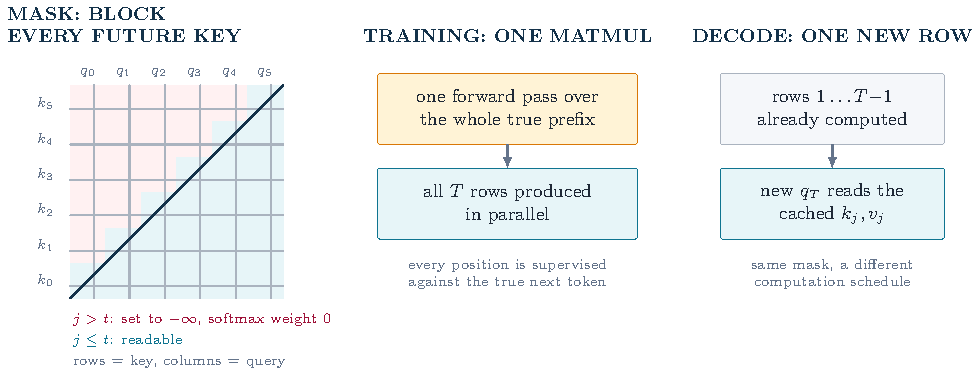
\includegraphics[width=0.6\textwidth]{causal_mask.pdf}
  \vfill
  \begin{columns}[T]
    \begin{column}{0.55\textwidth}
      \begin{concept}{独立和的方差}
        $q,k$ 各分量独立、均值 0、方差 1 时 $\mathrm{Var}(q\cdot k)=d_k$；除以 $\sqrt{d_k}$ 让 logit 方差为 1，softmax 不会过早饱和。
      \end{concept}
    \end{column}
    \begin{column}{0.42\textwidth}
      \small
      因果 mask 让位置 $t$ 只看见 $x_{\le t}$：一次矩阵乘法给出所有位置的预测，标签不会泄漏。
    \end{column}
  \end{columns}
\end{frame}

\begin{frame}{多头与位置}
  \begin{columns}[T]
    \begin{column}{0.5\textwidth}
      \textbf{多头注意力}
      \[
        \mathrm{MHA}(X)=\mathrm{Concat}(\mathrm{head}_1,\ldots,\mathrm{head}_h)\,W_O
      \]
      每个 head 有自己的 $W_Q,W_K,W_V$，在各自子空间里用不同的相似度检索：有的看语法搭配，有的看指代，有的看相邻位置。$W_O$ 把各 head 的结果混合回残差流。
      \vspace{2mm}

      \textbf{位置信息}\quad 注意力只看内容，打乱 token 顺序结果不变；必须另外注入位置。
    \end{column}
    \begin{column}{0.47\textwidth}
      \centering
      \begin{tikzpicture}[x=1mm,y=1mm]
        \draw[GSlate!40] (0,0) circle (16);
        \draw[GSlate!40] (-19,0) -- (19,0);
        \draw[GSlate!40] (0,-19) -- (0,19);
        \draw[-{Latex[length=1.8mm]},GOrange,line width=1.1pt] (0,0) -- (25:15);
        \draw[-{Latex[length=1.8mm]},GTeal,line width=1.1pt] (0,0) -- (80:15);
        \node[lblo,anchor=west] at (25:16) {$R_mq$};
        \node[lblt,anchor=south] at (80:16) {$R_nk$};
        \draw[GNavy,-{Latex[length=1.2mm]}] (25:7) arc (25:80:7);
        \node[lbln] at (52:10.5) {$(n-m)\theta$};
      \end{tikzpicture}
      \par\vspace{2mm}
      {\small \textbf{RoPE}（旋转位置编码）：把 $q,k$ 每两维看作平面向量，在位置 $m$ 旋转角度 $m\theta$。内积 $(R_mq)^\top(R_nk)=q^\top R_{n-m}k$ 只依赖相对位置 $n-m$。}
    \end{column}
  \end{columns}
\end{frame}

\begin{frame}{一个 Transformer block}
  \begin{columns}[c]
    \begin{column}{0.68\textwidth}
      \centering
      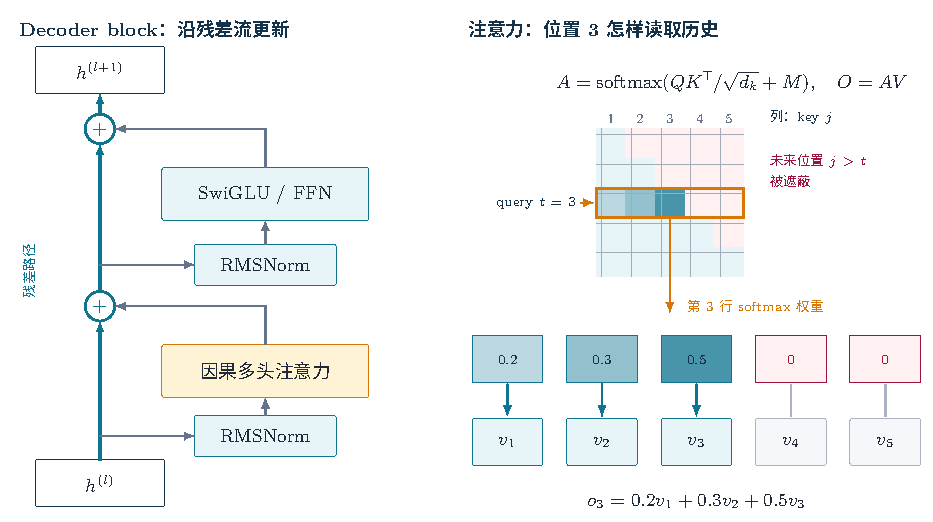
\includegraphics[width=\linewidth]{transformer_block_detailed.pdf}
    \end{column}
    \begin{column}{0.3\textwidth}
      \small
      \begin{itemize}
        \item \textbf{残差流}：$h\leftarrow h+\mathcal F(\mathrm{Norm}(h))$，每个子层只写入一个增量，深层也能稳定训练
        \item \textbf{注意力}在位置之间交换信息
        \item \textbf{FFN}（前馈网络）在每个位置内部做非线性特征变换
        \item \textbf{归一化}把每个 token 的向量调到稳定尺度
      \end{itemize}
      一个 block 堆叠 $L$ 次（几十到上百层）。
    \end{column}
  \end{columns}
\end{frame}

\begin{frame}{从最后一层到下一个 token 的分布}
  \begin{columns}[c]
    \begin{column}{0.5\textwidth}
      \centering
      \begin{tikzpicture}[x=1mm,y=1mm]
        \foreach \i/\w in {0/BOS,1/猫,2/坐,3/在}{%
          \node[nsoft,minimum width=9mm,font=\scriptsize] (in\i) at (\i*13,0) {\w};
          \node[nteal,minimum width=9mm,minimum height=5mm,font=\scriptsize] (e\i) at (\i*13,9) {$e$};
          \draw[ar] (in\i) -- (e\i);}
        \node[nnavy,minimum width=50mm,minimum height=9mm] (blk) at (19.5,21) {$L$ 个 block（因果注意力 + FFN）};
        \foreach \i in {0,...,3}{\draw[ar] (e\i) -- (\i*13,16.5);}
        \foreach \i/\w in {0/猫,1/坐,2/在,3/垫子}{%
          \node[norange,minimum width=9mm,minimum height=5mm,font=\scriptsize] (o\i) at (\i*13,33) {$p_\theta$};
          \draw[ar] (\i*13,25.5) -- (o\i);
          \node[font=\scriptsize,text=GOrange] at (\i*13,39) {\w};}
        \node[lbl,anchor=west] at (46,39) {标签};
        \node[lbl,anchor=west] at (46,33) {softmax$(W h_t)$};
        \node[lbl,anchor=west] at (46,0) {输入};
      \end{tikzpicture}
    \end{column}
    \begin{column}{0.47\textwidth}
      \[
        p_\theta(x_{t+1}=v\mid x_{\le t})=\softmax\bigl(Wh_t^{(L)}\bigr)_v
      \]
      \begin{itemize}
        \item \textbf{训练}：整段真实文本一次送入，每个位置都与下一个 token 计算交叉熵，即第二讲的极大似然
        \item \textbf{生成}：抽出一个 token 接到末尾，再算下一个位置；必须串行
        \item \textbf{KV cache}（键值缓存）：前缀各位置的 $k,v$ 不会再变，生成时缓存起来，每步只算新位置
      \end{itemize}
    \end{column}
  \end{columns}
\end{frame}

\begin{frame}{三种结构，三种条件分布}
  \centering
  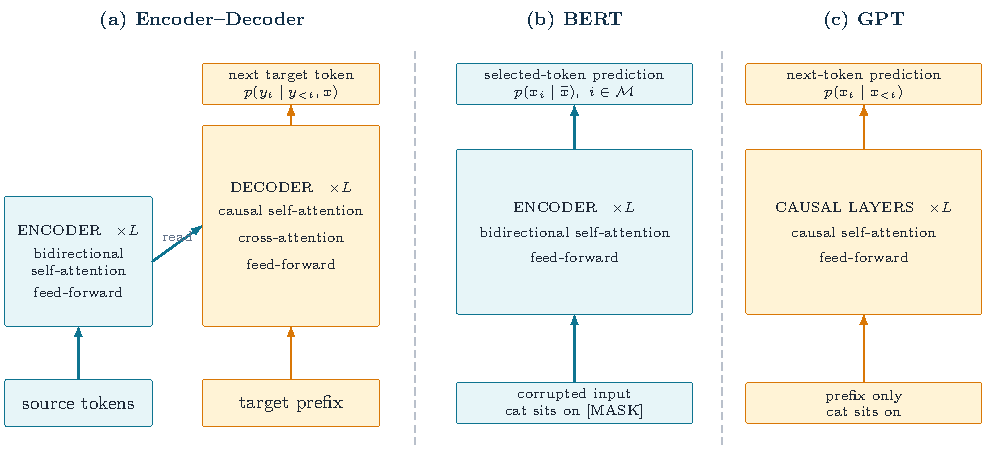
\includegraphics[width=0.7\textwidth]{transformer_overview.pdf}
  \vfill
  \small
  \begin{tabularx}{\textwidth}{@{}>{\color{GNavy}\bfseries}l l X@{}}
    \toprule
    结构 & 学习的分布 & 用途\\
    \midrule
    Encoder--Decoder & $p(y_t\mid y_{<t},x)$ & 翻译等“读完再写”的任务\\
    BERT & $p(x_i\mid\tilde x)$：遮住一些词再猜回 & 双向编码器：文本表示、分类、检索\\
    GPT & $p(x_t\mid x_{<t})$：预测下一个 token & 生成式预训练：续写、对话、大语言模型\\
    \bottomrule
  \end{tabularx}
\end{frame}

% ====================================================================
\section{大模型的训练阶段}

\begin{frame}{从续写到对话，再到推理}
  \centering
  \begin{tikzpicture}[x=1mm,y=1mm]
    \node[draw=GTeal,fill=GSky,rounded corners=2pt,text width=37mm,minimum height=44mm,align=left,inner sep=2.5mm,font=\small] (a) at (0,0) {\textbf{1. 预训练：学会续写}\\[1.5mm]预测下一个 token\\[1mm]{\ttfamily\footnotesize Q: 1+1? A: 2\\Q: 3+3? A:}\\[1mm]{\scriptsize\color{GSlate}数万亿 token 的网页、书籍、代码}};
    \node[draw=GNavy,fill=GMist,rounded corners=2pt,text width=37mm,minimum height=44mm,align=left,inner sep=2.5mm,font=\small] (b) at (48,0) {\textbf{2. 对齐：学会回答}\\[1.5mm]SFT（监督微调）：示范“合格回答”\\RLHF（基于人类反馈的强化学习）：人类比较两个回答的好坏\\[1mm]{\scriptsize\color{GSlate}用户：提问\quad 助手：回答}};
    \node[draw=GOrange,fill=GAmber,rounded corners=2pt,text width=37mm,minimum height=44mm,align=left,inner sep=2.5mm,font=\small] (c) at (96,0) {\textbf{3. 推理：学会多想}\\[1.5mm]RLVR（可验证奖励的强化学习）：程序判定答案对错，奖励正确的解题过程\\[1mm]{\ttfamily\footnotesize <think>…</think>}\\{\scriptsize\color{GSlate}数学、代码等可验证任务}};
    \draw[ar,line width=1pt] (a.east) -- (b.west);
    \draw[ar,line width=1pt] (b.east) -- (c.west);
  \end{tikzpicture}
  \vfill
  \begin{takeaway}
    三个阶段用的是同一个自回归模型 $\prod_tp_\theta(x_t\mid x_{<t})$，改变的是：经验分布由谁提供，以及目标里有没有奖励。
  \end{takeaway}
\end{frame}

\begin{frame}{预训练与 SFT：同一个极大似然}
  \begin{columns}[T]
    \begin{column}{0.5\textwidth}
      \textbf{预训练}\quad 在语料经验分布 $\hat\pi$ 上最小化负对数似然（NLL），即 $\KL(\hat\pi\Vert p_\theta)$
      \begin{itemize}
        \item 数据配比 $\hat\pi=\sum_k\alpha_k\hat\pi_k$（网页、代码、数学、多语言……）本身就是在选择目标分布
        \item 参数量、数据量、算力需要按 scaling law 配平
      \end{itemize}
      \vspace{1mm}
      \textbf{SFT}\quad 换成“指令 $c$ + 合格回答 $y$”的数据，损失只在回答 token 上计算：
      \[
        \mathcal L_{\mathrm{SFT}}=-\E_{(c,y)}\sum_t\log p_\theta(y_t\mid y_{<t},c)
      \]
    \end{column}
    \begin{column}{0.47\textwidth}
      \begin{concept}{经验分布与混合分布}
        预训练和 SFT 的差别只在 $\hat\pi$：前者覆盖所有文本，后者集中在“回答问题”这一小部分。
      \end{concept}
      \vspace{1mm}
      \begin{caution}[SFT 的局限]只有正例：模型学到“这样回答可以”，却学不到“另一种回答差多少”。比较好坏需要奖励或偏好。\end{caution}
    \end{column}
  \end{columns}
\end{frame}

\begin{frame}{RLHF：在参考分布附近提高奖励}
  \begin{columns}[T]
    \begin{column}{0.55\textwidth}
      给回答打分的奖励 $r(x)$ 来自人类偏好训练的奖励模型或程序判题器。目标：提高奖励，又不远离参考模型 $p_0$（通常是 SFT 模型）。
      \begin{keystep}
        \keyeq{
          \E_q[r]-\tau\KL(q\Vert p_0)
          &=-\tau\,\E_q\Bigl[\log q-\log p_0-\tfrac{r}{\tau}\Bigr]\\
          &=-\tau\,\KL(q\Vert q^*)+\tau\log Z}
        所以最优策略是 $q^*=p_0\,e^{r/\tau}/Z$。
      \end{keystep}
      \begin{concept}{玻尔兹曼分布与自由能}
        奖励是负能量，$\tau$ 是温度，$p_0$ 是先验测度；目标就是第一讲的变分自由能。
      \end{concept}
    \end{column}
    \begin{column}{0.42\textwidth}
      \begin{tikzpicture}
        \begin{axis}[genai,width=6.4cm,height=4.6cm,xmin=-3,xmax=4,ymin=0,ymax=0.72,xtick=\empty,ytick=\empty,xlabel={回答空间（示意）},domain=-3:4,samples=241,legend style={at={(0.02,0.98)},anchor=north west}]
          \addplot[GSlate,fill=GSlate!15] {(0.7*exp(-(x+1)^2/0.72)+0.3*exp(-(x-1.5)^2/0.72))/(0.6*sqrt(2*pi))} \closedcycle;
          \addlegendentry{$p_0$}
          \addplot[GTeal] {(0.401*exp(-(x+0.82)^2/0.72)+0.599*exp(-(x-1.68)^2/0.72))/(0.6*sqrt(2*pi))};
          \addlegendentry{$\tau=2$}
          \addplot[GOrange] {(0.161*exp(-(x+0.64)^2/0.72)+0.839*exp(-(x-1.86)^2/0.72))/(0.6*sqrt(2*pi))};
          \addlegendentry{$\tau=1$}
        \end{axis}
      \end{tikzpicture}
      \par{\scriptsize\slate{奖励 $r(x)=x$：$\tau$ 越小，概率越向高奖励一侧移动；但只能在 $p_0$ 已有质量的地方重新分配}}
    \end{column}
  \end{columns}
\end{frame}

\begin{frame}{奖励怎样传回每个 token}
  \begin{columns}[T]
    \begin{column}{0.53\textwidth}
      回答 $y$ 是逐 token 抽出的离散序列，梯度不能穿过抽样，用 score-function 估计：
      \[
        \nabla_\theta\E_{y\sim\pi_\theta}[r]=\E\Bigl[(r-b)\sum_t\nabla_\theta\log\pi_\theta(y_t\mid y_{<t},c)\Bigr]
      \]
      \small
      \begin{tabularx}{\linewidth}{@{}>{\color{GNavy}\bfseries}l X@{}}
        \toprule
        PPO & 近端策略优化：另训一个价值网络作基线 $b$，每个位置的优势不同\\
        GRPO & 组相对策略优化：同一题采样一组回答，以组内平均分作基线\\
        DPO & 直接偏好优化：不在线采样，直接用“好 / 差”回答对拟合 $q^*$\\
        \bottomrule
      \end{tabularx}
      \begin{concept}{score-function 估计}
        由 $\nabla_\theta\pi_\theta=\pi_\theta\nabla_\theta\log\pi_\theta$ 得到，只要 $\log\pi_\theta$ 可微，离散的 $y$ 也适用；基线 $b$ 不改变期望，只降低方差。
      \end{concept}
    \end{column}
    \begin{column}{0.44\textwidth}
      \centering
      \begin{tikzpicture}[x=1mm,y=1mm]
        \node[nsoft,minimum width=20mm] (p) at (0,30) {题目 $c$};
        \foreach \i/\r in {0/1,1/0,2/1,3/0}{%
          \node[nteal,minimum width=11mm,minimum height=6mm,font=\scriptsize] (y\i) at (\i*14-21,16) {$y_{\i}$};
          \draw[ar] (p.south) -- (y\i.north);
          \node[font=\scriptsize,text=GInk] at (\i*14-21,9) {$r=\r$};}
        \draw[GSlate!60] (-29,0) -- (29,0);
        \foreach \i/\a in {0/1,1/-1,2/1,3/-1}{%
          \pgfmathsetmacro{\col}{\a>0?1:0}
          \ifdim\col pt>0.5pt \fill[GTeal] (\i*14-24,0) rectangle ++(6,5);\else\fill[GRose] (\i*14-24,0) rectangle ++(6,-5);\fi}
        \node[lbl,anchor=north] at (0,-7) {优势 $A_i=r_i-\bar r$（组内平均 $\bar r=0.5$）};
      \end{tikzpicture}
      \par\vspace{2mm}
      {\small GRPO：答对的整条轨迹各 token 概率被抬高，答错的被压低。}
    \end{column}
  \end{columns}
\end{frame}

\begin{frame}{想一想：没人教它验算}
  \begin{columns}[c]
    \begin{column}{0.5\textwidth}
      RLVR：不示范解题步骤，只让程序判最后答案的对错，对给 1 分，错给 0 分。训练一段时间后，回答越来越长，模型开始自己写出这样的话：
      \vspace{3mm}
      \begin{tcolorbox}[genaibox,colback=GMist,colframe=GMist,fontupper=\footnotesize]
        ……所以 $x=12$。\par
        等等，我再验算一下：代回原式，左边是 $30$，右边是 $32$，不对。\par
        回到第二步重新算……
      \end{tcolorbox}
      {\scriptsize\slate{示意}}
    \end{column}
    \begin{column}{0.46\textwidth}
      \begin{hook}
        \opt{1}{没人教过它验算。这种行为是从哪里来的？}
        \opt{2}{RL 是教会了模型新的解题方法，还是做了别的事？}
      \end{hook}
    \end{column}
  \end{columns}
\end{frame}

\begin{frame}{推理模型：RLVR 与思维链}
  \begin{columns}[T]
    \begin{column}{0.53\textwidth}
      回答 $y=(z,a)$：先写推理链 $z$，再给答案 $a$。数学、代码可由程序判对错：$r(y)=\mathbf 1[a\text{ 正确}]$。
      \begin{itemize}
        \item 目标 $\E_{\pi_\theta}[r]=\sum_z\pi_\theta(z\mid c)\,P(a\text{ 对}\mid z,c)$：推理链像隐变量一样被求和；奖励只看答案，不需要标注解题步骤
        \item 用上一页的 GRPO 训练：答对的整条推理链被抬高
        \item 训练中回答变长，自发出现验算、回退（OpenAI o1，2024；DeepSeek-R1，2025）。多写的 token 就是额外的串行计算
      \end{itemize}
      \begin{caution}[局限]
        判题器要可靠；只看答案时，过程可能是碰对的。$p_0$ 几乎不写的推理方式很难被采到，也就很难得到奖励。
      \end{caution}
    \end{column}
    \begin{column}{0.44\textwidth}
      \centering
      \begin{tikzpicture}
        \begin{axis}[genai,ybar,bar width=4pt,width=6.3cm,height=3.3cm,ymin=0,ymax=0.65,ytick={0,0.3,0.6},xtick={1,...,6},xticklabels={{$z_1$\\错},{$z_2$\\对},{$z_3$\\错},{$z_4$\\错},{$z_5$\\对},{$z_6$\\对}},xticklabel style={align=center},enlarge x limits=0.12,every axis plot/.append style={line width=0.4pt}]
          \addplot[draw=GSlate,fill=GSlate!35] coordinates {(1,0.30) (2,0.22) (3,0.18) (4,0.14) (5,0.10) (6,0.06)};
          \addplot[draw=GTeal,fill=GTeal!60] coordinates {(1,0.181) (2,0.362) (3,0.109) (4,0.085) (5,0.164) (6,0.099)};
          \addplot[draw=GOrange,fill=GOrange!70] coordinates {(1,0) (2,0.579) (3,0) (4,0) (5,0.263) (6,0.158)};
        \end{axis}
      \end{tikzpicture}
      \par\vspace{1mm}
      {\scriptsize\slate{六条推理链：\textcolor{GSlate}{灰}为 $p_0$，\teal{青}为 $\tau=1$，\orange{橙}为 $\tau\to0$。$p_0$ 下答对的概率是 $0.38$}}
      \vspace{2mm}
      \begin{concept}{条件概率}
        代入 RLHF 页的 $q^*=p_0e^{r/\tau}/Z$，$r$ 只取 0 或 1：
        \keyeq{q^*(y)\propto p_0(y)\,e^{r(y)/\tau}\,\xrightarrow{\tau\to0}\,p_0(y\mid\text{答对})}
        答对的链按原有相对概率放大 $1/0.38$ 倍，答错的被剔除。
      \end{concept}
    \end{column}
  \end{columns}
\end{frame}

\begin{frame}{RL 教会了模型什么}
  \begin{answer}[回到问题 1]
    验算、回退在 $p_0$ 的输出里本来就偶尔出现。带验算的链更常答对，奖励把它们一轮轮放大，回答也随之变长。DeepSeek-R1-Zero 的论文把训练中途出现的这种“等等，再想想”称作 aha moment。
  \end{answer}
  \vspace{2mm}
  \begin{answer}[回到问题 2]
    主要是重新分配概率。上一页 $\tau\to0$ 时 $q^*=p_0(y\mid\text{答对})$：答对的链按原有比例放大，$p_0$ 几乎不写的推理方式很难被采到。实验上也有迹象：允许采样很多次时（pass@$k$，即 $k$ 次采样中至少一次做对的比例，$k$ 很大），RL 之后的模型能做对的题并不比基座模型多（Yue 等，2025）。
  \end{answer}
  \vfill
  \begin{takeaway}
    RL 更像是把“偶尔做对”变成“稳定做对”。目标仍是第一讲的变分自由能：在先验 $p_0$ 附近，按奖励重新加权。
  \end{takeaway}
\end{frame}

% ====================================================================
\begin{frame}{全课回顾：六条路线}
  \centering
  \input{figures/genmap.tex}
  \vfill
  {\small Transformer 是第一张卡片里的条件分布网络；扩散模型的去噪网络也常用它。大模型的后训练回到第一讲的自由能。}
\end{frame}

\begin{frame}{全课小结}
  \begin{takeaway}[带走的几件事]
    \begin{enumerate}
      \item 生成模型的核心问题只有一个：用样本学一个高维分布，并能从中抽样；难点集中在归一化常数 $Z$
      \item 训练目标都是分布之间的差距：极大似然是前向 KL，变分推断与 RLHF 是反向 KL（自由能），GAN 是 JSD，score matching 是 Fisher 散度
      \item 各类模型的区别在怎样处理 $Z$：分解、变换、下界、放弃密度、只用比值、只用梯度
      \item 扩散把一次困难的采样拆成许多次简单的去噪；关键一步是“噪声回归学到的后验平均恰好就是 score”
      \item 大语言模型 $=$ 链式法则 $+$ Transformer $+$ 极大似然，再用带 KL 约束的奖励优化做对齐
    \end{enumerate}
  \end{takeaway}
\end{frame}

\appendix
\section{附录}

\begin{frame}{附录：反向扩散与 Langevin，像在哪，不同在哪}
  \begin{columns}[T]
    \begin{column}{0.48\textwidth}
      \begin{keystep}[换成 score 的写法]
        代入 $\epsilon_\theta=-b_ts_t$，采样的一步是
        \keyeq{x_{t-1}=\frac{x_t+\beta_t\,s_t(x_t)}{\sqrt{\alpha_t}}+\sigma_tz}
        第二讲的 Langevin 是
        \keyeq{x\leftarrow x+\tfrac{\eta}{2}\,s(x)+\sqrt{\eta}\,z}
        形式相同：沿 score 走一步，再加高斯噪声。
      \end{keystep}
      \begin{concept}{拆开看}
        步长小时 $\sigma_t^2\approx\beta_t$。忽略 $\sqrt{\alpha_t}$ 的缩放，一步的增量拆成两半：
        \keyeq{\beta_ts_t+\sqrt{\beta_t}\,z=\underbrace{\tfrac12\beta_ts_t+\sqrt{\beta_t}\,z}_{\eta=\beta_t\text{ 的 Langevin}}+\underbrace{\tfrac12\beta_ts_t}_{\text{确定性输运}}}
        前一半只在 $p_t$ 内部搅动，不改变分布；后一半把 $p_t$ 推向 $p_{t-1}$，就是正文的概率流 ODE。
      \end{concept}
    \end{column}
    \begin{column}{0.49\textwidth}
      \small
      \begin{tabularx}{\linewidth}{@{}>{\color{GNavy}\bfseries}l X X@{}}
        \toprule
        & Langevin & 反向扩散\\
        \midrule
        目标 & 一个固定的 $p$ & 一串分布 $p_T\to p_0$\\
        score & 每步相同 & 每步换成 $s_t$\\
        每一步 & 保持 $p$ 不变 & 把 $p_t$ 变成 $p_{t-1}$\\
        步数 & 等链混合，事先不知 & 正好 $T$ 步\\
        多峰 & 卡在一个峰里 & 高噪声时峰已连通\\
        \bottomrule
      \end{tabularx}
      \vspace{3mm}
      \begin{takeaway}
        Langevin 在一个固定分布里反复游走，要等它混合；反向扩散每一步都换一个分布，顺着 $p_T\to\cdots\to p_0$ 走下来，走完 $T$ 步就是数据的样本。
      \end{takeaway}
    \end{column}
  \end{columns}
\end{frame}

\begin{frame}{附录：一个统一的图景}
  \centering
  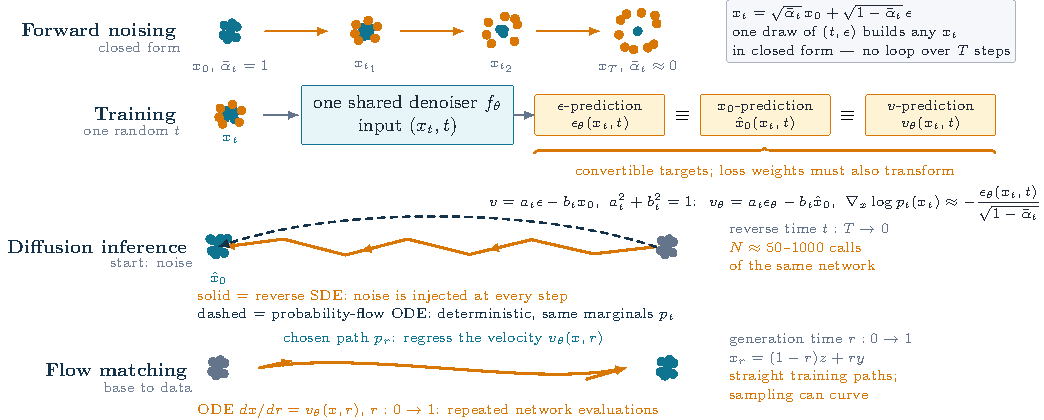
\includegraphics[width=0.78\textwidth]{diffusion_score_flow_paths.pdf}
  \vfill
  \begin{takeaway}
    DDPM 学噪声（等价于 score），用随机的反向转移生成；同一个网络也可以沿概率流 ODE 确定性地大步采样（见后面的 DDIM 页）；Flow Matching 直接学选定路径上的速度。在高斯路径上，噪声、干净样本、score 与速度可以互相换算，差别在路径、损失权重和求解器。
  \end{takeaway}
\end{frame}

\begin{frame}{附录：为什么回归条件速度就够了}
  \begin{columns}[T]
    \begin{column}{0.56\textwidth}
      \begin{keystep}[三步]
        \textbf{条件路径}：固定数据点 $y$，路径 $x_r=(1-r)z+ry$ 的速度 $u_r(x\mid y)=\frac{y-x}{1-r}$ 已知，条件密度 $p_r(x\mid y)$ 满足连续性方程。

        \smallskip
        \textbf{叠加}：令 $v_r(x)=\E[y-z\mid x_r=x]$，则
        \keyeq{p_r(x)\,v_r(x)=\int p_{\mathrm{data}}(y)\,p_r(x\mid y)\,u_r(x\mid y)\,dy}
        对 $y$ 积分条件连续性方程，得 $\partial_rp_r+\nabla\cdot(p_rv_r)=0$：$v_r$ 把 $\mathcal N(0,I)$ 恰好搬运成 $p_{\mathrm{data}}$。

        \smallskip
        \textbf{损失分解}：
        \keyeq{\E\bigl\|v_\theta-(y-z)\bigr\|^2=\E\bigl\|v_\theta-v_r(x_r)\bigr\|^2+C}
      \end{keystep}
    \end{column}
    \begin{column}{0.41\textwidth}
      同一个技巧在正文出现了两次：把不可算的边缘目标换成可算的条件目标。
      \begin{itemize}
        \item \textbf{扩散}：边缘 score $\nabla\log p_t(x)$\\$\to$ 条件 score $-\epsilon/b_t$
        \item \textbf{流}：边缘速度 $v_r(x)$\\$\to$ 条件速度 $y-z$
      \end{itemize}
      \vspace{1mm}
      \begin{concept}{条件期望}
        均方误差下，对条件目标回归与对边缘目标回归只差一个与参数无关的常数，最优解相同。
      \end{concept}
    \end{column}
  \end{columns}
\end{frame}

\begin{frame}{附录：DDIM（去噪扩散隐式模型），同一个网络，更少的步数}
  \begin{columns}[T]
    \begin{column}{0.52\textwidth}
      在当前 $x_t$ 调用一次网络，先估计干净样本，再按更早时刻 $s<t$ 的系数重新组合：
      \[
        \begin{aligned}
          \hat x_0&=\frac{x_t-b_t\,\epsilon_\theta(x_t,t)}{a_t},\\
          x_s&=a_s\hat x_0+b_s\,\epsilon_\theta(x_t,t)
        \end{aligned}
      \]
      \begin{itemize}
        \item 训练不变，只改采样器；不再注入新噪声，相当于沿概率流 ODE 走大步
        \item 1000 步训练调度，生成时只取 50 个时刻
        \item 更好的 ODE 求解器、蒸馏等方法还能进一步压到几步
      \end{itemize}
    \end{column}
    \begin{column}{0.45\textwidth}
      \centering
      \begin{tikzpicture}[x=0.86mm,y=1mm]
        \draw[GSlate!50] (0,14) -- (62,14);
        \foreach \i in {0,...,40}{\draw[GSlate!60] (\i*1.5,13) -- (\i*1.5,15);}
        \node[lbl,anchor=east] at (-1,14) {DDPM};
        \draw[GSlate!50] (0,2) -- (62,2);
        \foreach \i in {0,8,...,40}{\fill[GTeal] (\i*1.5,2) circle (0.9);}
        \foreach \i in {0,8,16,24,32}{\draw[arteal] (60-1.5*\i,5) to[bend right=40] (48-1.5*\i,5);}
        \node[lbl,anchor=east] at (-1,2) {DDIM};
        \node[lbl,anchor=north] at (60,0) {$T$};
        \node[lbl,anchor=north] at (0,0) {$0$};
      \end{tikzpicture}
      \par\vspace{3mm}
      \begin{takeaway}
        扩散的计算成本主要来自步数；训练出的 score 网络可以配不同的采样器。
      \end{takeaway}
    \end{column}
  \end{columns}
\end{frame}

\begin{frame}{附录：条件生成，classifier-free guidance}
  \begin{columns}[T]
    \begin{column}{0.52\textwidth}
      训练时随机丢掉一部分样本的条件 $c$（如文本描述），同一个网络既能给出 $\epsilon_\theta(x_t,t,c)$，也能给出 $\epsilon_\theta(x_t,t,\varnothing)$。采样时
      \[
        \epsilon_{\mathrm{guide}}=\epsilon_{\mathrm{uncond}}+w\,(\epsilon_{\mathrm{cond}}-\epsilon_{\mathrm{uncond}})
      \]
      \begin{concept}{贝叶斯公式}
        $\nabla\log p(x\mid c)=\nabla\log p(x)+\nabla\log p(c\mid x)$。引导相当于从 $p(x)\,p(c\mid x)^w$ 采样：$w>1$ 把似然放大，样本更贴合条件，多样性下降。
      \end{concept}
    \end{column}
    \begin{column}{0.45\textwidth}
      \centering
      \begin{tikzpicture}[x=1mm,y=1mm]
        \pgfmathsetseed{21}
        \foreach \sx/\t/\sp in {0/{$w=1$}/4.5,32/{$w=4$}/2}{%
          \begin{scope}[shift={(\sx,0)}]
            \draw[GSlate!50] (0,0) rectangle (28,28);
            \foreach \cx/\cy in {7/20,21/21,9/7}{\foreach \j in {1,...,8}{\fill[GSlate!45] (\cx+3.5*rand,\cy+3.5*rand) circle (0.55);}}
            \foreach \j in {1,...,12}{\fill[GTeal] (20+\sp*rand,8+\sp*rand) circle (0.6);}
            \node[lbl,anchor=north] at (14,-1) {\t};
          \end{scope}}
        \node[lblt,anchor=north,text width=60mm] at (30,-6) {青色：条件 $c$ 下的样本；灰色：其他类别};
      \end{tikzpicture}
      \par\vspace{3mm}
      {\small 文生图模型中的“提示词相关度”参数就是 $w$；每步需要两次网络调用。}
    \end{column}
  \end{columns}
\end{frame}

\end{document}
